This chapter describes the methodology adopted to achieve the project goals. It summarizes the main steps, details the implementation choices, and specifies the experimental protocol so the study can be reproduced.

\section{General Idea}

The project aims to use AI to guide an FM synthesizer to simulate any target timbre. In practical terms, a CNN receives a raw audio sample and predicts a set of FM parameters that can re-synthesize the same sound, allowing the synthesizer to emulate an instrument playing musical sounds (or even emulate not musical sounds).

To operationalize this idea, the methodology follows the steps below:

\begin{enumerate}
  \item Implement a simple FM synthesizer suitable for controlled data generation and evaluation.
  \item Generate a synthetic dataset of audio samples and corresponding parameter values.
  \item Train a CNN regressor to predict synthesizer parameters from raw audio.
  \item Evaluate generalization using the Google NSynth dataset and objective audio similarity metrics.
\end{enumerate}

FM synthesis was selected because it offers expressive timbral control at low computational cost, yet requires expert knowledge to tune. Then, learning parameter mappings with a neural model reduces manual effort (of a trial-and-error process) while enables fast and repeatable synthesis.

All experiments were conducted on the following software and hardware environment:

\begin{itemize}
  \item Python 3.11.2
  \item TensorFlow 2.19.0
  \item Keras 3.11.1
  \item NVIDIA CUDA 12.5.82
  \item cuDNN 3.0.75
  \item NVIDIA driver 535.247.01
  \item CUDA toolkit 12.2
  \item NVIDIA GeForce GTX 1650 GPU with 4 GB of memory
\end{itemize}

\section{Implementing the FM Synthesizer}
\label{sec:fm_synth}

There are several commercial FM synthesizers with hundreds or thousands of parameters. However, this work focuses on a research-oriented, controllable baseline. Therefore, a deliberately simple synthesizer was implemented to validate the overall pipeline.

Commercial synthesizers can expose extremely large parameter spaces. For example, Native Instruments' FM8 can use around 1,000 parameters, while the Teenage Engineering OP-1 has been described as reaching up to $10^{76}$ possible parameter combinations \cite{claesson2021resynthesis}. These figures reinforce why a simplified synthesizer is useful in this study: it keeps the experimentation tractable while still exercising the main FM synthesis concepts.

\begin{figure}[h]
  \centering
  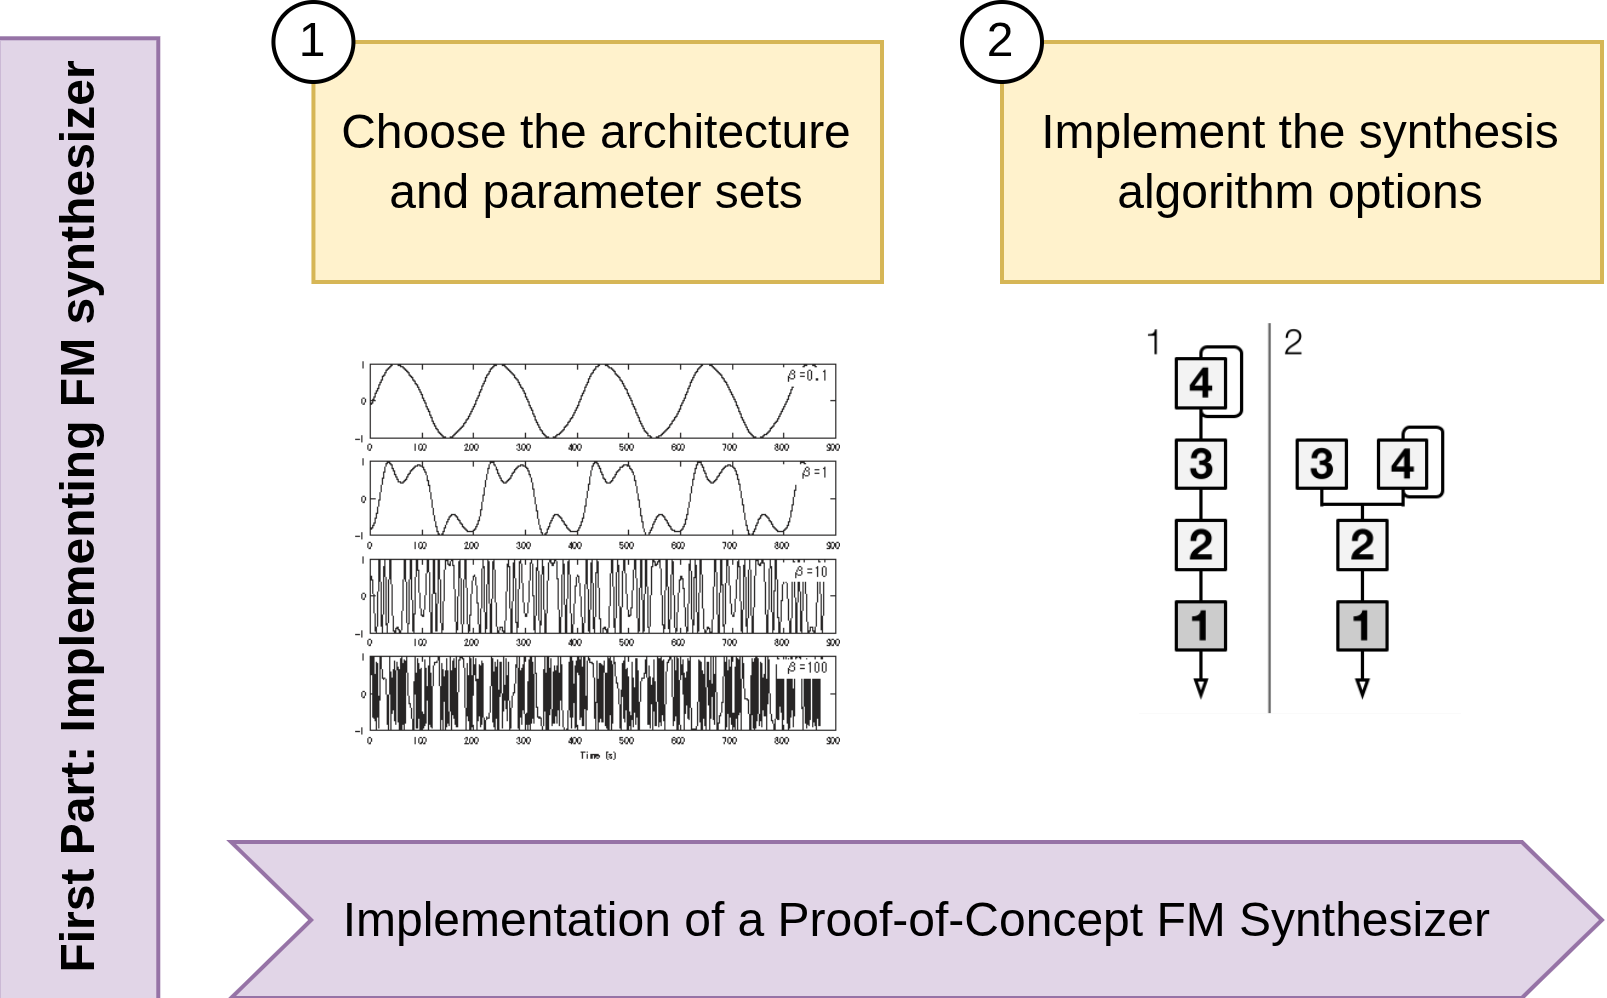
\includegraphics[width=0.9\linewidth]{../images/first_part.png}
  \caption{Overview of the synthesis implementation.}
  \label{fig:met1}
\end{figure}

The implemented synthesizer uses 6 (six) operators inspired by the Yamaha DX7 and supports two algorithms (one fully serial and one mixed serial/parallel). It contains 5 modulator operators, 1 carrier operator, and a single ADSR envelope. The two operator topologies are shown in Figure~\ref{fig:FMSynth}.

\begin{figure}[h]
  \centering
  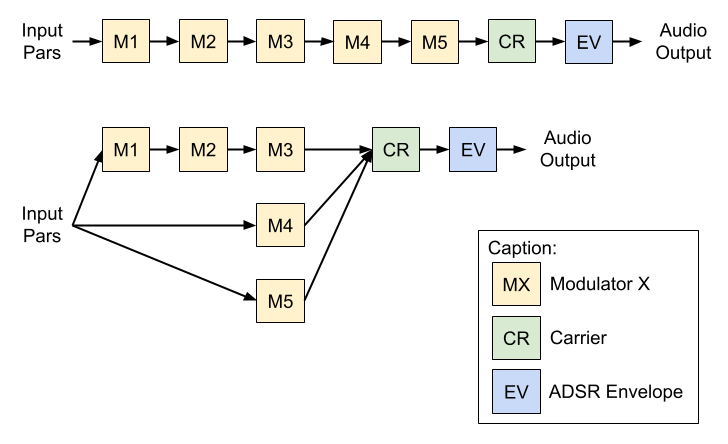
\includegraphics[width=0.85\linewidth]{../images/algs2.png}
  \caption{FM synthesizer operator algorithms.}
  \label{fig:FMSynth}
\end{figure}

The synthesis pipeline follows four steps:

\begin{enumerate}
  \item Generate each operator signal by phase modulation of the next operator in the chain.
  \item Combine operator outputs according to the selected algorithm (parallel outputs are summed).
  \item Apply the ADSR envelope.
  \item Downsample from 48 kHz to 16 kHz with a low-pass filter to avoid aliasing.
\end{enumerate}

A 48 kHz internal rate was used to reduce aliasing caused by high-frequency components generated by FM operators. Downsampling is performed with low-pass filtering to maintain stability and avoid wrong spectral artifacts.

The synthesizer exposes 16 parameters: 12 parameters for ratios and modulation indices (beta) across the five modulators and the carrier, plus 4 ADSR parameters (attack, decay, sustain, release). This configuration is intentionally minimal yet sufficient to cover the FM principles needed for the study.

\section{Datasets}
\label{sec:datasets}

Two datasets are used: a synthetic dataset for training and a real-instrument dataset (NSynth) for evaluation.

\subsection{Synthetic dataset}

The synthetic dataset is built by sampling FM parameters and rendering the corresponding audio. This produces explicit tuples of (parameters, audio), enabling supervised training of the CNN/regressor. The parameter sampling strategy follows prior FM resynthesis work that constrains the search space to musically plausible ranges while still exploring diverse timbres \cite{claesson2021resynthesis}.

\begin{figure}[h]
  \centering
  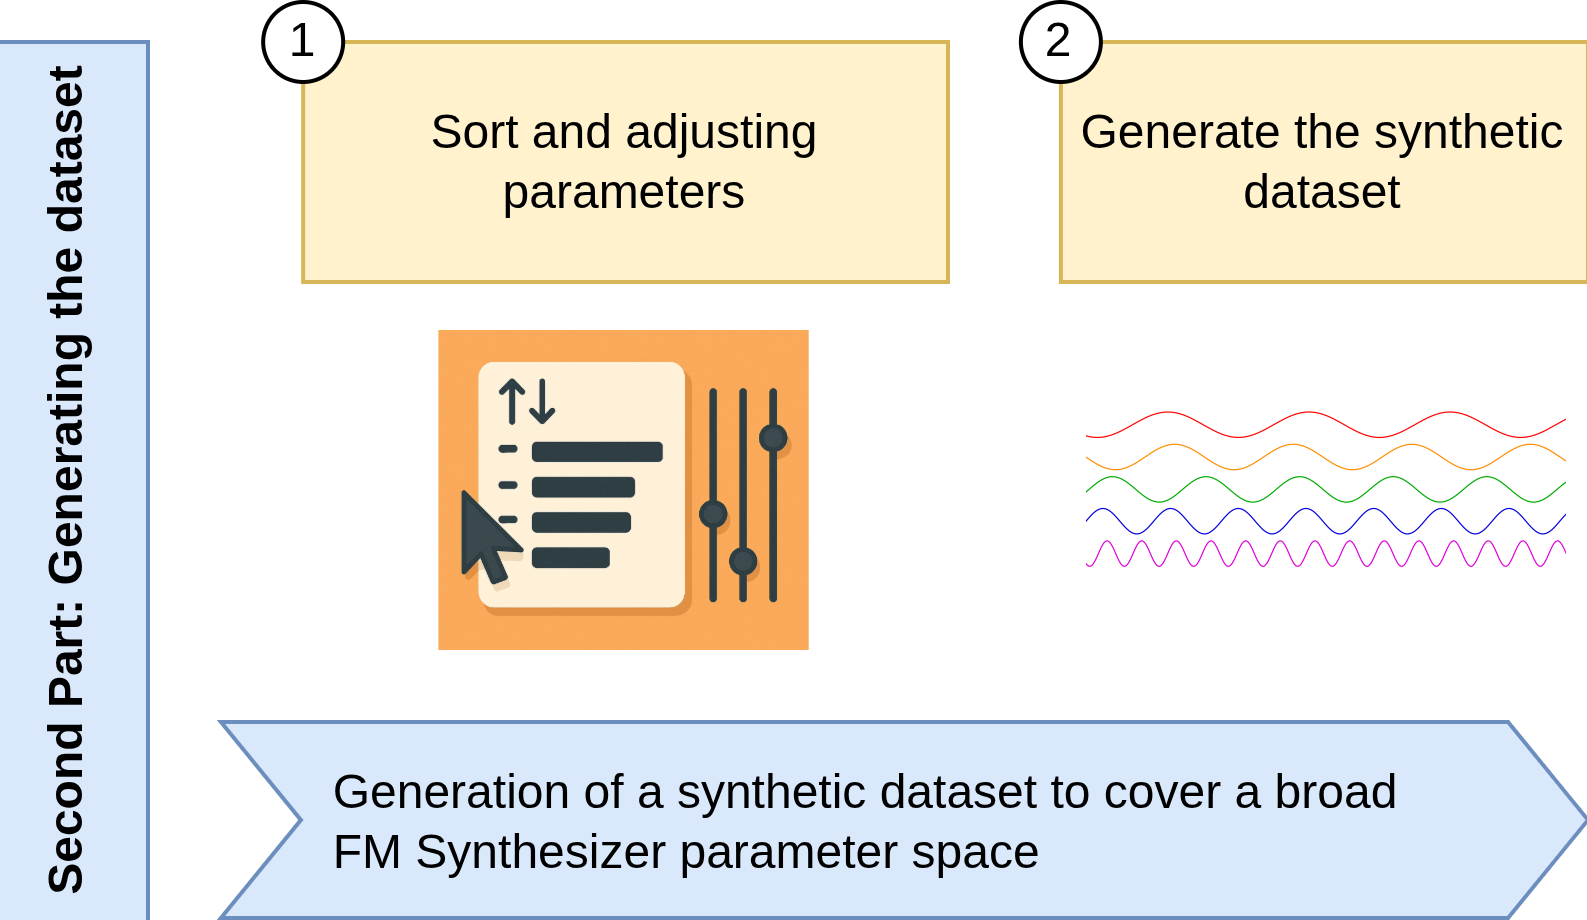
\includegraphics[width=0.9\linewidth]{../images/second_part.png}
  \caption{Synthetic dataset generation overview.}
  \label{fig:met2}
\end{figure}

Each sample is 4 seconds long, monophonic, and stored at 16 kHz (signals are generated at 48 kHz and then downsampled for compatibility with NSynth dataset). The dataset contains 5,000 samples, with pitches between 20 Hz and 6 kHz and randomized ADSR envelopes.

To make the random samples musically plausible and reduce aliasing, the following constraints were applied:

\begin{itemize}
  \item Carrier frequency is drawn uniformly from 20 Hz to 6 kHz, keeping the highest base frequencies below the Nyquist limit after downsampling.
  \item Modulator ratios are constrained to the range [1/8, 8]. With 90\% probability the ratio is drawn from a discrete harmonic-like set; with 10\% probability it is drawn from a log-uniform distribution to allow metallic timbres \cite{chowning1973synthesis,nielsen2020practical}.
  \item Modulation indices (beta) are drawn uniformly in [0, 8] with a biased distribution: 20\% in [0, 0.5], 60\% in [0.5, 3], and 20\% in [3, 8], prioritizing rich but stable timbres and increasing sideband count and spectral bandwidth as the index grows \cite{chowning1973synthesis,nielsen2020practical}.
  \item Amplitude is fixed at 1.0 to avoid parameter redundancies that yield identical spectra.
  \item ADSR parameters are sampled from uniform intervals: attack in [0.005, 0.5] s, decay in [0.02, 0.6] s, sustain in [0.1, 0.9], and release in [0.05, 0.8] s.
\end{itemize}

The dataset is split into 3,750 training samples and 1,250 test samples. From the training split, 20\% is reserved for validation, resulting in 3,000 training and 750 validation samples.

\subsection{External dataset (NSynth)}

The NSynth dataset from Google Magenta project contains real instrument samples and is used to evaluate generalization \cite{engel2017nsynth}. Only the test subset is used during evaluation, with:

\begin{itemize}
  \item 4,096 samples;
  \item 4 seconds per sample;
  \item 16 kHz sampling rate;
  \item 11 instrument families;
  \item pitches from 27.5 Hz to 4,186.01 Hz.
\end{itemize}

\section{Training the CNN}
\label{sec:training_cnn}

The mapping from audio to FM parameters is not analytically tractable, because each operator introduces additional spectral components. Therefore, this work learns the mapping from raw waveforms using a CNN-based regressor.

\begin{figure}[h]
  \centering
  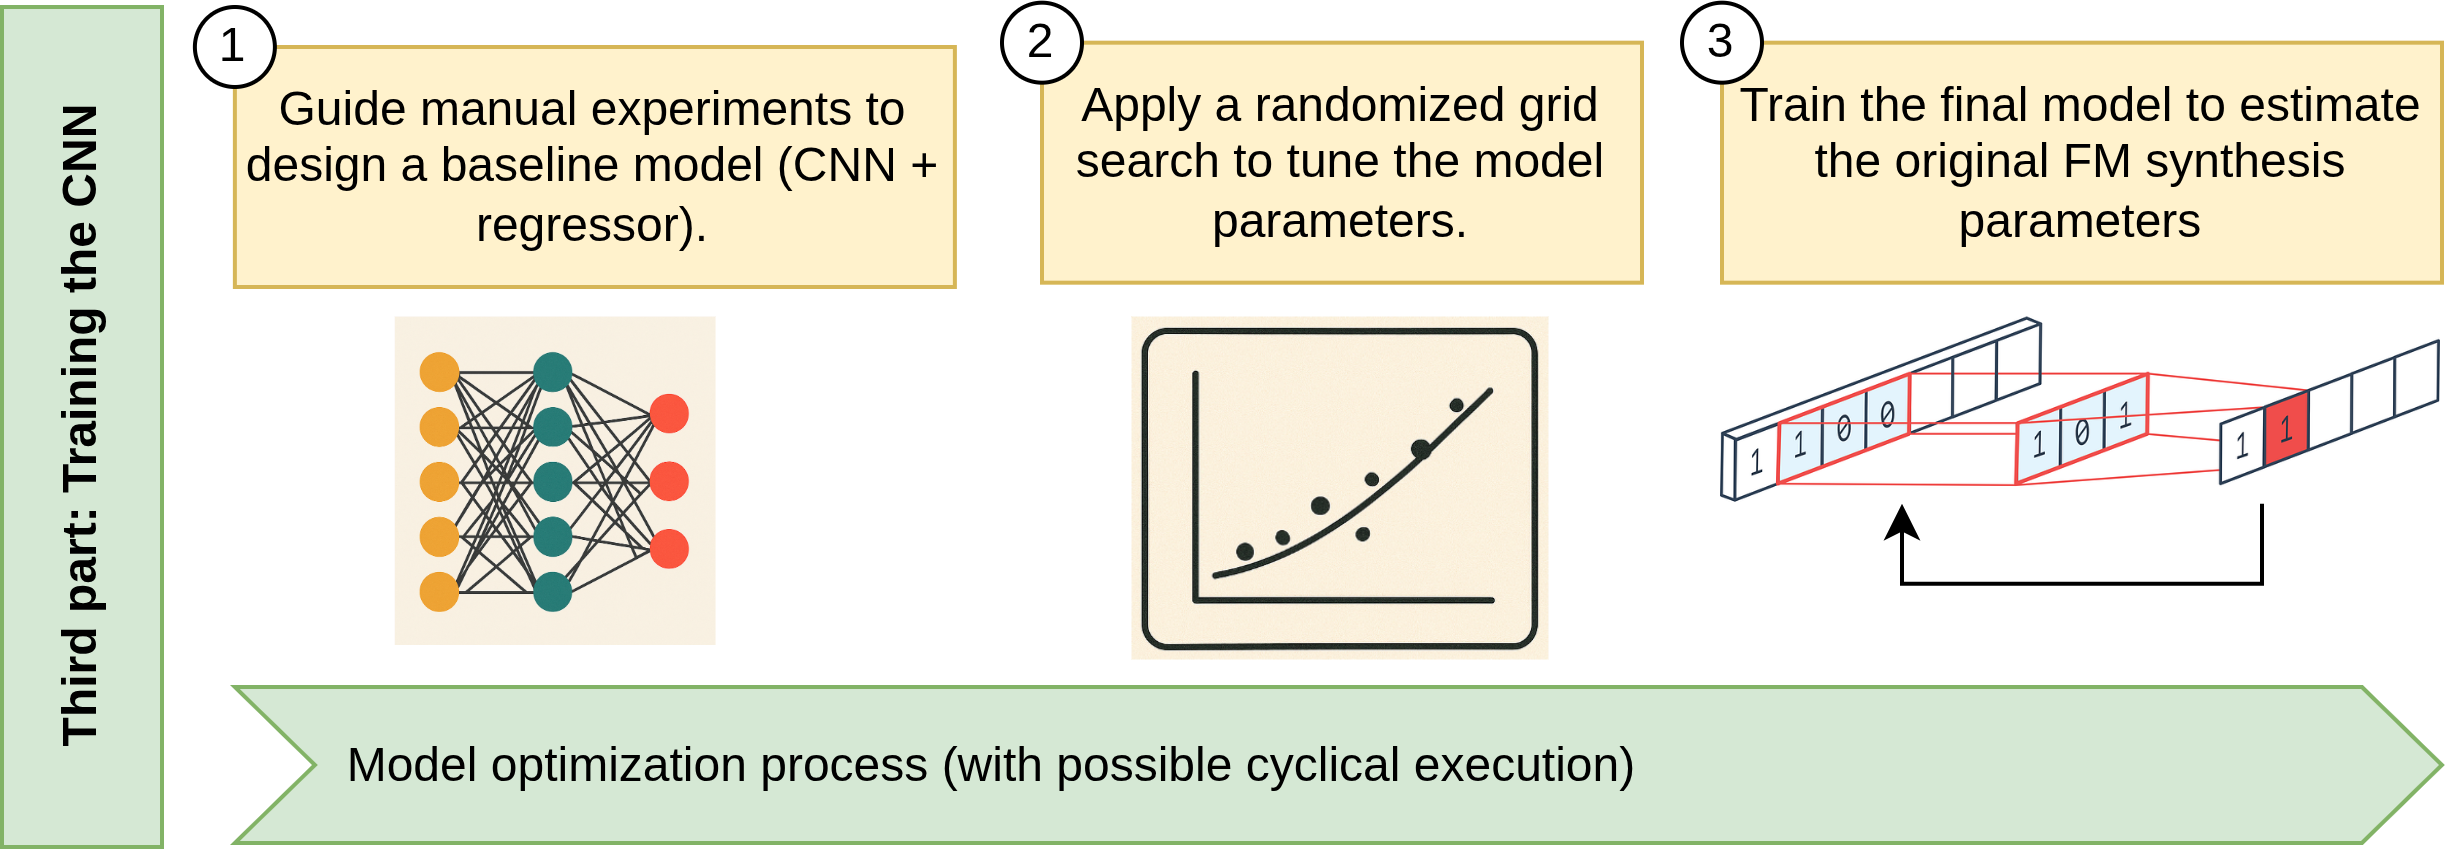
\includegraphics[width=0.9\linewidth]{../images/thrid_part.png}
  \caption{Model training and optimization overview.}
  \label{fig:met3}
\end{figure}

\subsection{Model architecture}

The model combines a CNN-based feature extractor with a fully connected regressor. Figure~\ref{fig:redes} summarizes the two modules.

\begin{figure}[h]
  \centering
  \begin{subfigure}[b]{0.45\textwidth}
    \centering
    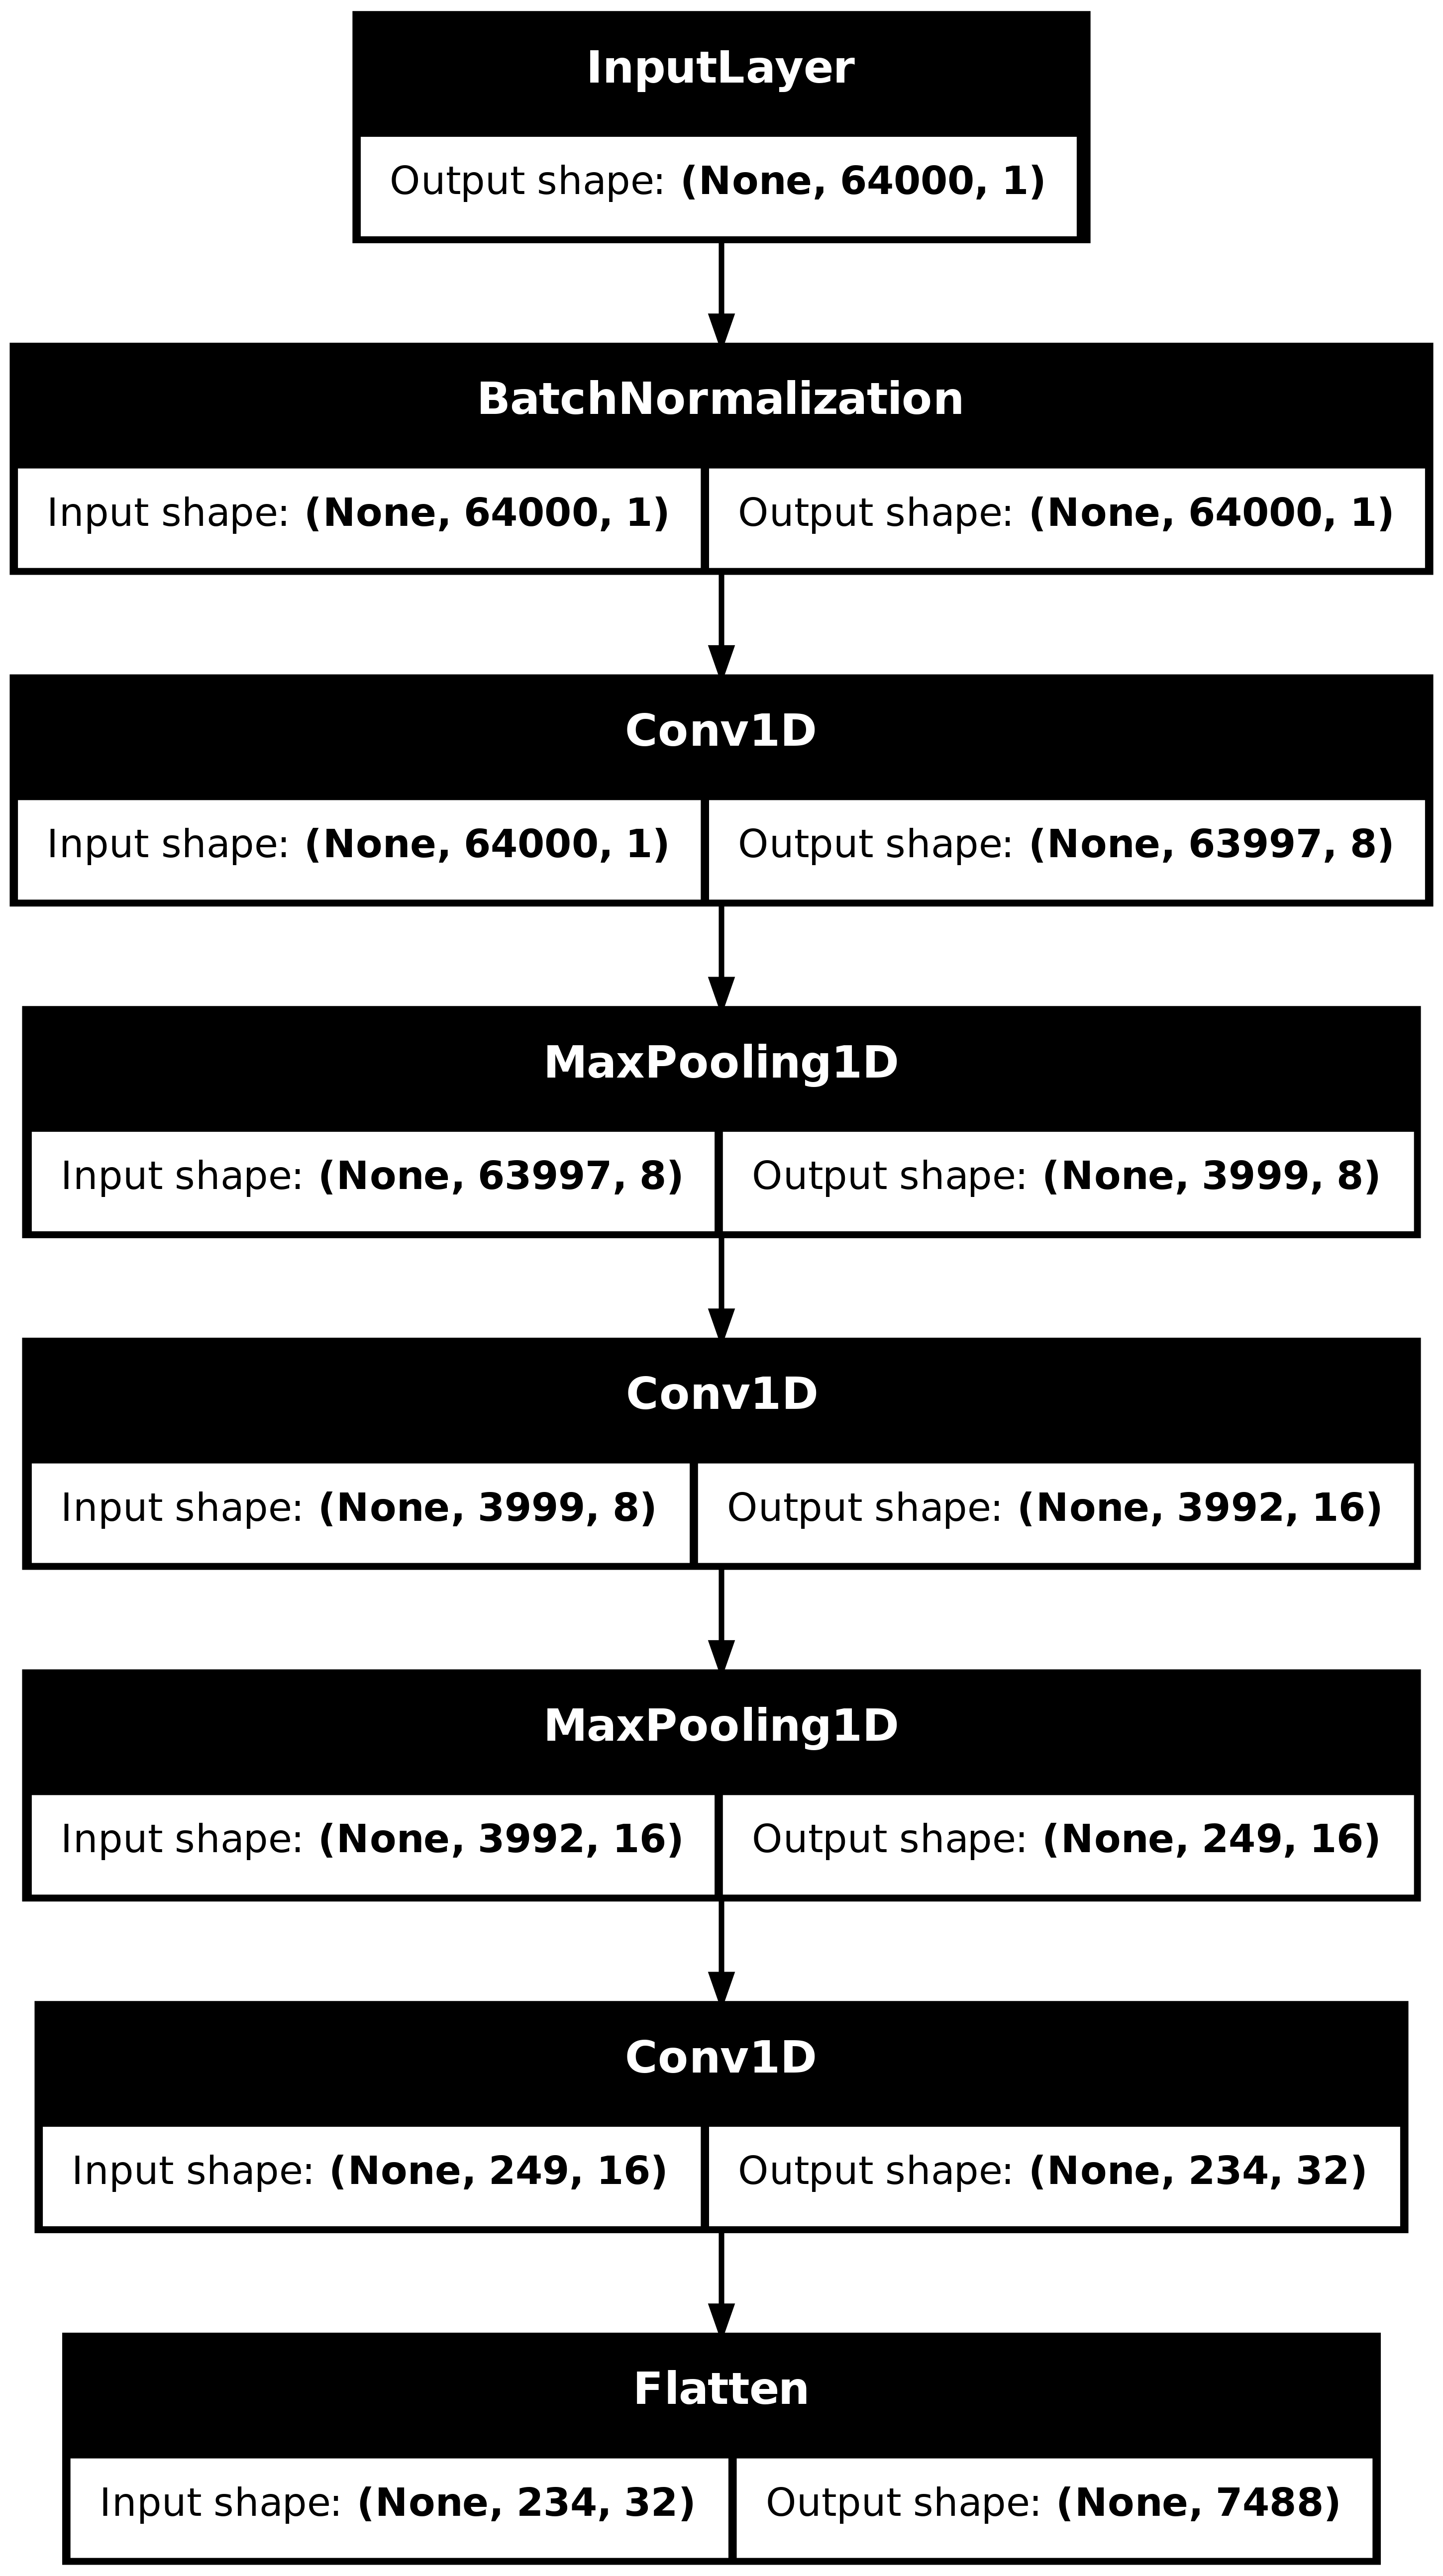
\includegraphics[width=\textwidth,height=0.4\textwidth,trim={0 0 0 0.6cm},clip]{../images/rede1.png}
    \caption{Feature extraction}
    \label{fig:rede1}
  \end{subfigure}
  \hfill
  \begin{subfigure}[b]{0.45\textwidth}
    \centering
    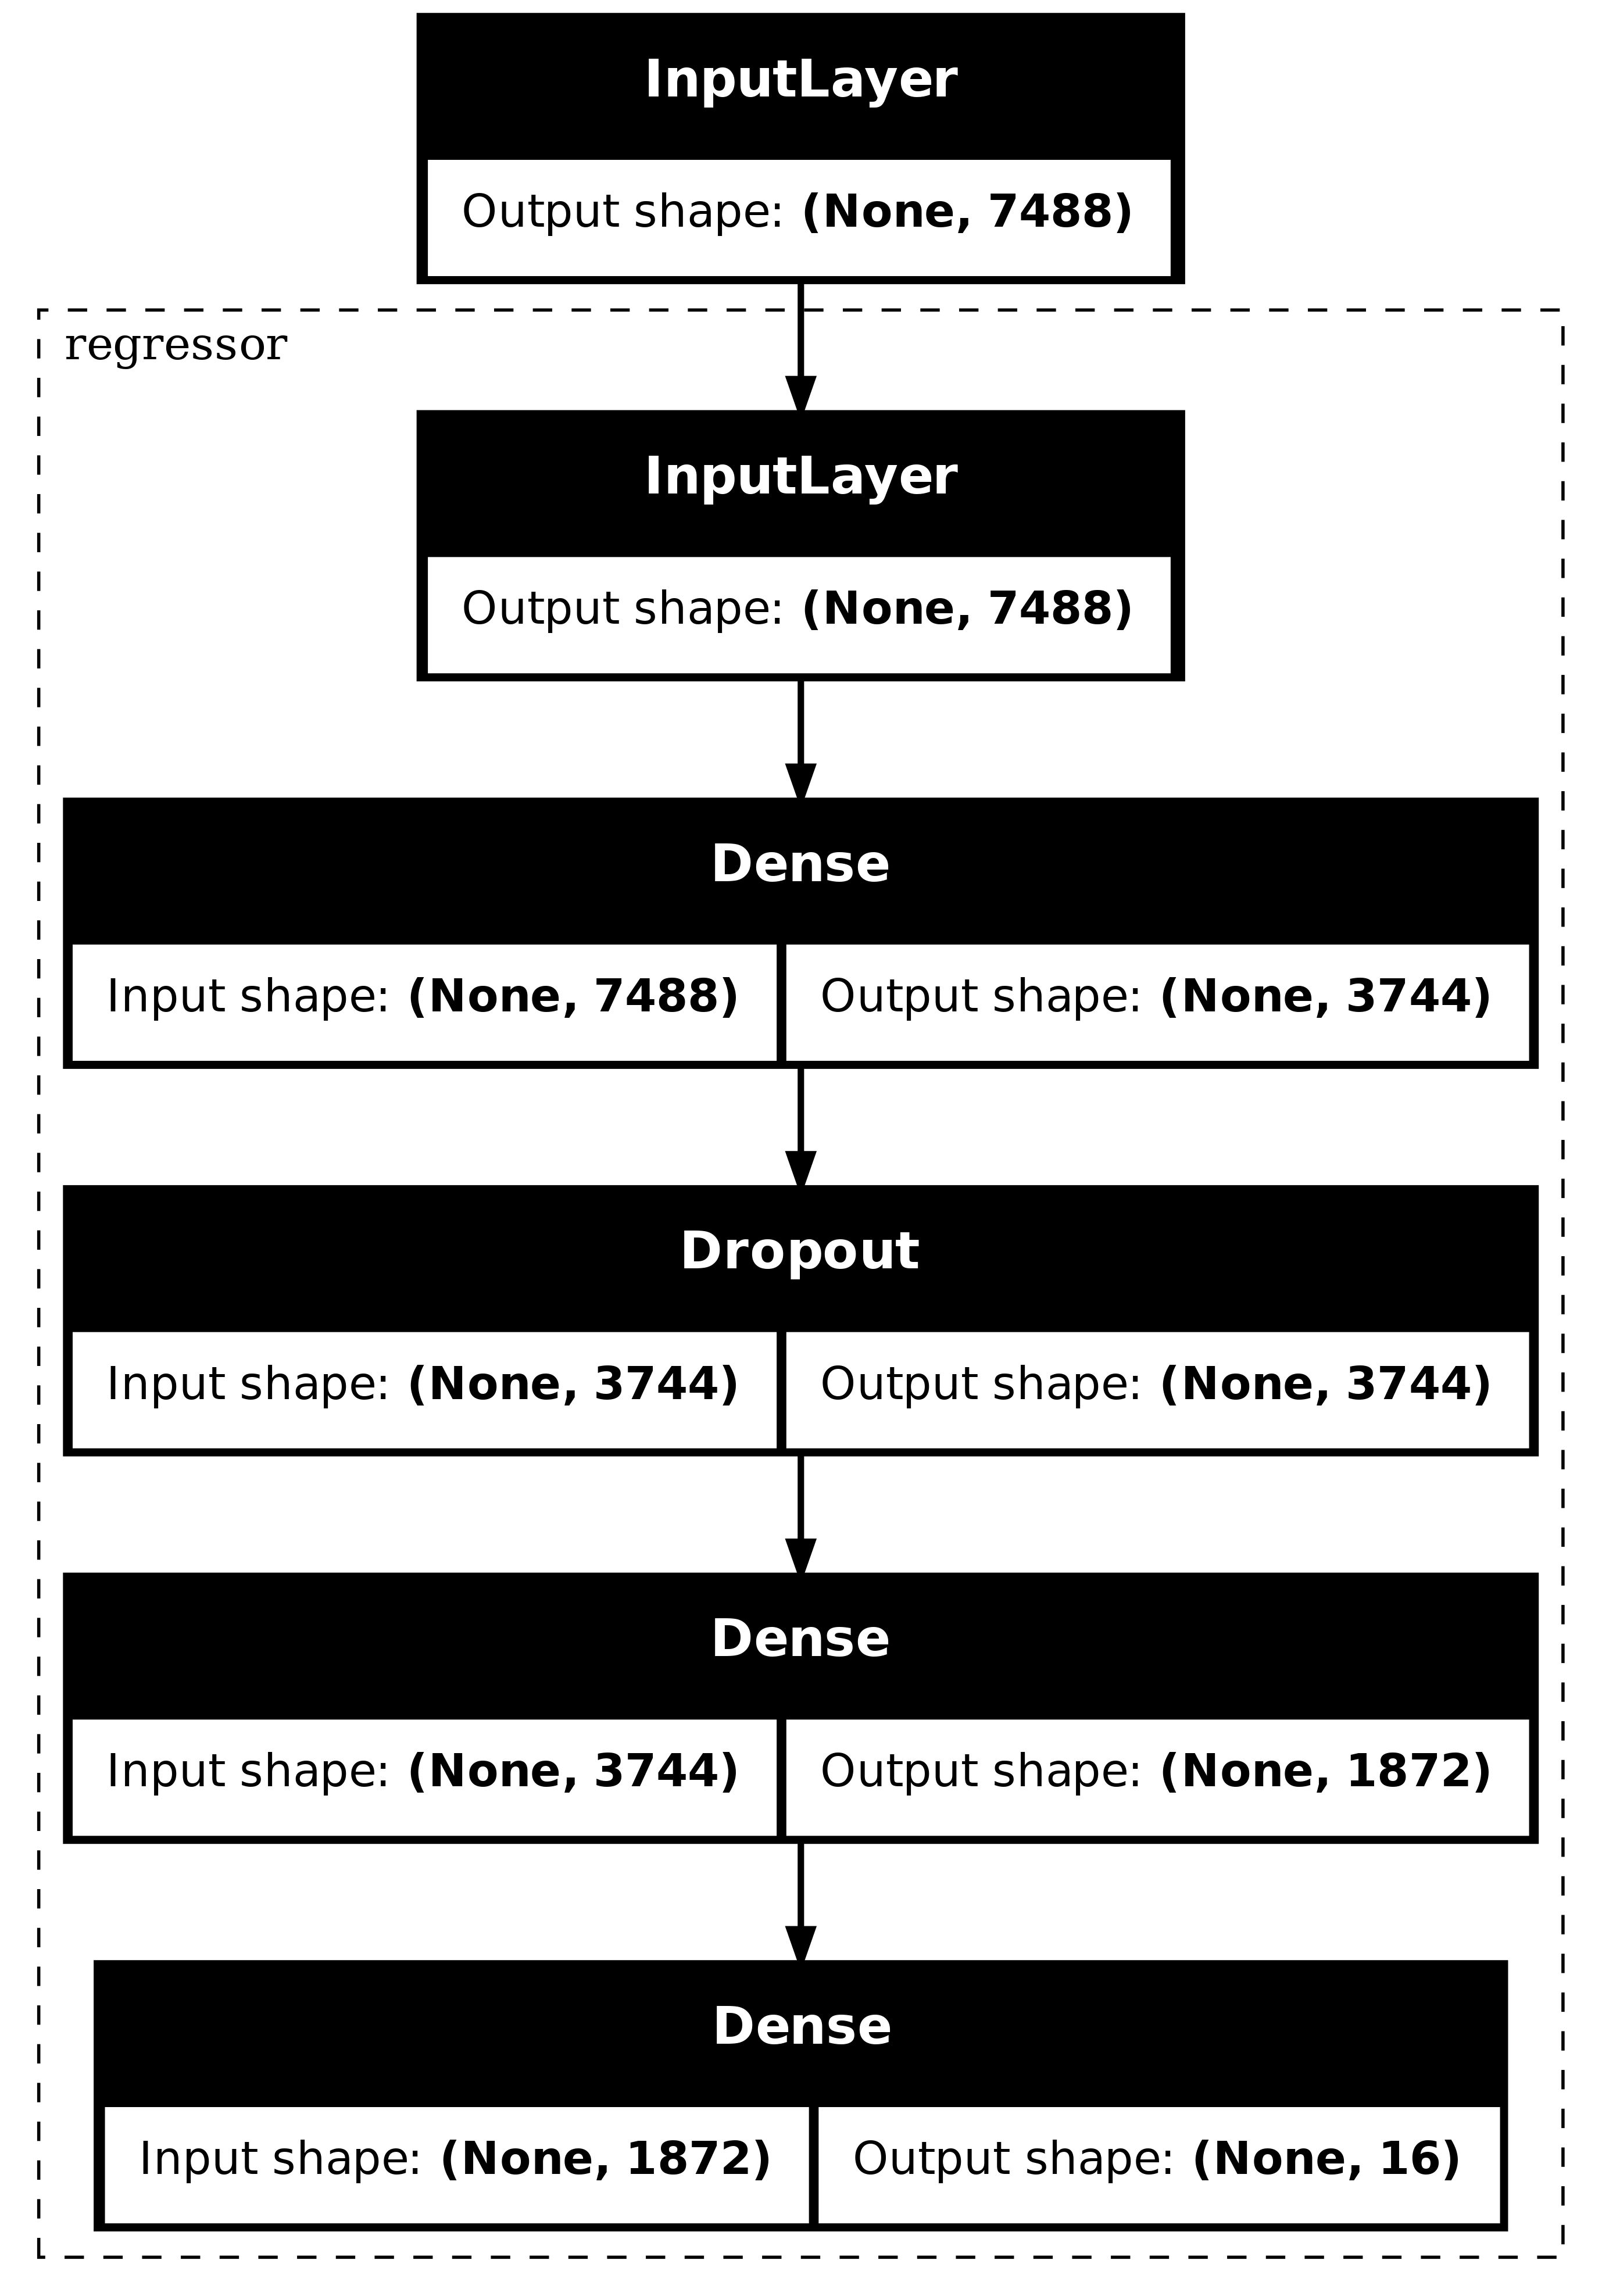
\includegraphics[width=\textwidth,height=0.4\textwidth,trim={0 0 0 0.85cm},clip]{../images/rede2.png}
    \caption{Regressor}
    \label{fig:rede2}
  \end{subfigure}
  \caption{Overview of the CNN feature extractor and regressor.}
  \label{fig:redes}
\end{figure}

The CNN uses three Conv1D–MaxPooling blocks, while the regressor uses two dense layers and a linear output. The hyperparameters are summarized in Tables~\ref{tab:hyperparams_cnn} and \ref{tab:hyperparams_regressor}.

\begin{table}[htb] \small \centering
  \caption{Hyperparameters of the CNN feature extractor}
  \label{tab:hyperparams_cnn}
  \begin{tabular}{l|l|l}
    \hline
    Component        & Hyperparameter            & Value       \\
    \hline
    Conv1D (1)       & Filters / Kernel / Stride & 8 / 4 / 1   \\
    MaxPooling1D (1) & Pool size                 & 16          \\
    Conv1D (2)       & Filters / Kernel / Stride & 16 / 8 / 1  \\
    MaxPooling1D (2) & Pool size                 & 16          \\
    Conv1D (3)       & Filters / Kernel / Stride & 32 / 16 / 1 \\
    MaxPooling1D (3) & Pool size                 & 16          \\
    \hline
  \end{tabular}
\end{table}

\begin{table}[htb] \small \centering
  \caption{Hyperparameters of the regressor network}
  \label{tab:hyperparams_regressor}
  \begin{tabular}{l|l|l}
    \hline
    Component      & Hyperparameter & Value  \\
    \hline
    Dense (1)      & Activation     & ReLU   \\
    Dropout        & Rate           & 0.5    \\
    Dense (2)      & Activation     & ReLU   \\
    Dense (Output) & Activation     & Linear \\
    Optimizer      & --             & Nadam  \\
    \hline
  \end{tabular}
\end{table}

Additional settings include:

\begin{itemize}
  \item target normalization (zero mean and unit variance);
  \item MSE as loss;
  \item MAE/MSE as metrics;
  \item batch size 32;
  \item early stopping with patience 20 and best-weight restoration;
  \item training ran for up to 200 epochs;
\end{itemize}

\subsection{Hyperparameter optimization}

A randomized grid search was used to explore a broad hyperparameter space without exhaustive testing. Table~\ref{tab:hyperparams_options} lists the options. The full grid contains 5,184 combinations; 186 experiments (about 3.6\%) were sampled, each trained for 30 epochs with early stopping (patience 5). MLflow was used to track metrics and compare configurations.

\begin{table}[htb] \small \centering
  \caption{Hyperparameter options used in randomized search}
  \label{tab:hyperparams_options}
  \begin{tabular}{l|l}
    \hline
    Hyperparameter               & Options                                      \\
    \hline
    Activation                   & gelu, swish, elu, relu, selu, silu           \\
    CNN bias                     & true, false                                  \\
    CNN kernel regularizer       & none, l1, l2                                 \\
    Regressor bias               & true, false                                  \\
    Regressor dropout            & 0, 0.2, 0.3, 0.5                             \\
    Regressor kernel regularizer & none, l1, l2                                 \\
    Optimizer                    & AdamW, RMSprop, Adam, Nadam, Adagrad, Adamax \\
    \hline
  \end{tabular}
\end{table}

\begin{figure}[h]
  \centering
  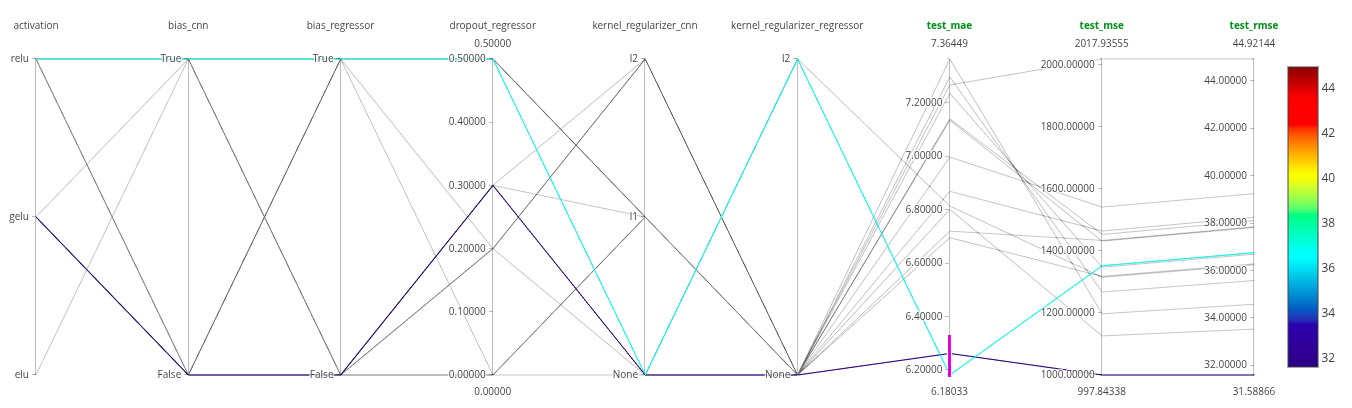
\includegraphics[width=\linewidth]{../images/graph_grid_search.png}
  \caption{MLflow grid search results for the sampled configurations.}
  \label{fig:graph}
\end{figure}

\section{Evaluation Method}
\label{sec:evaluation_method}

The NSynth test subset is used to evaluate generalization. Each NSynth sample is passed through the CNN to predict parameters, which are then applied to the synthesizer to re-synthesize the signal. The original and re-synthesized signals are compared with objective metrics.

\begin{figure}[h]
  \centering
  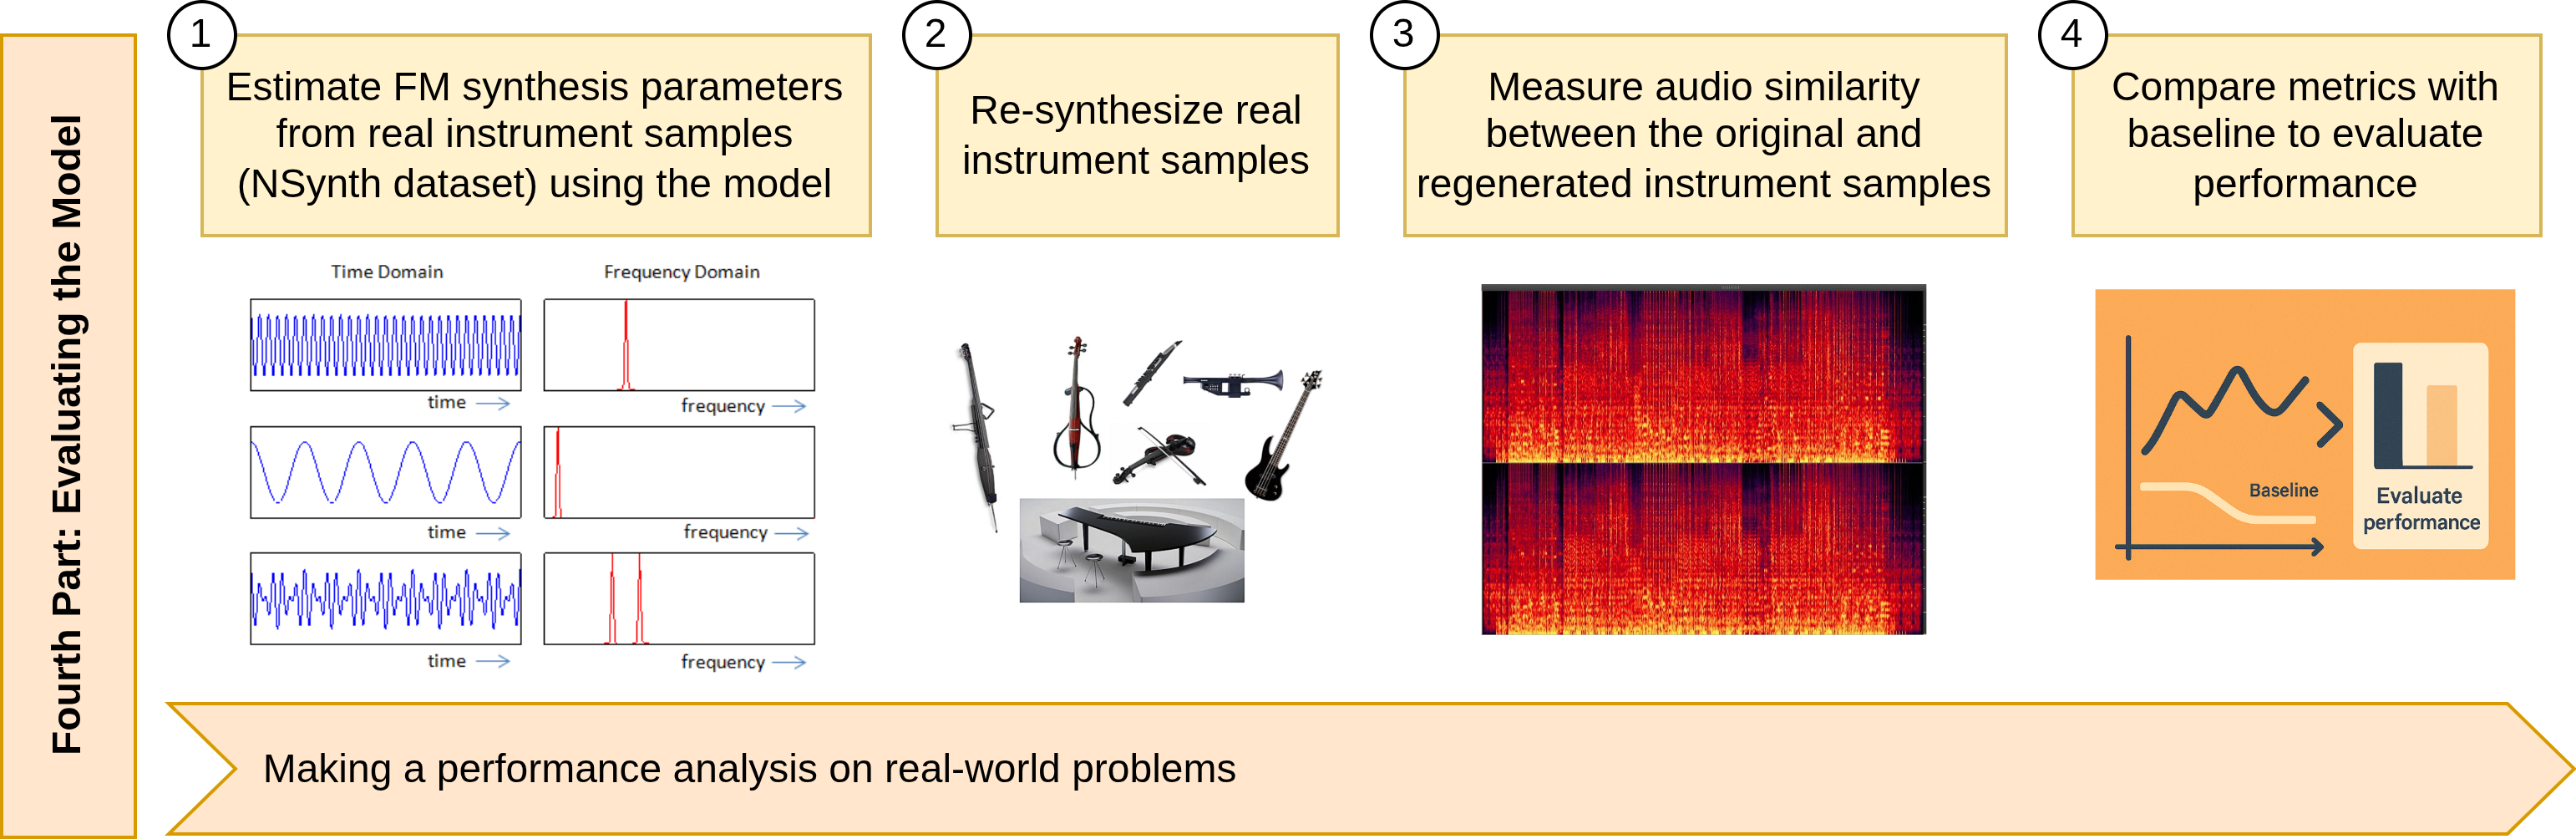
\includegraphics[width=0.9\linewidth]{../images/fourth_part.png}
  \caption{Evaluation workflow used for generalization testing.}
  \label{fig:met4}
\end{figure}

The evaluation uses FFT distance, STFT distance, and Log-Mel distance (raw and normalized). Before synthesis, ratio parameters are rounded to the nearest discrete harmonic values (matching the synthetic dataset), and parameters are clipped to the same bounds used in training. As a baseline, the same metrics are computed between each NSynth sample and a pure sinusoid at 440 Hz (A4).
